\documentclass{beamer}
\usepackage[utf8]{inputenc}
\usepackage[english]{babel}
\usepackage{graphicx}
\usepackage{hyperref}
\usepackage{listings}
\usepackage{xcolor}

% Définition du thème
\usetheme{Madrid}
\usecolortheme{dolphin}

% Informations sur la présentation
\title{IAASFIRECRACKER}
\subtitle{Infrastructure as a Service with Firecracker}
\author{\begin{columns}[T]
  \column{0.5\textwidth}
  ACHAIRE ZOGO \\
  TCHASSI DANIEL \\
  DONCHI TRESOR LEROY \\
  WANDJI Emmanuel
  \column{0.5\textwidth}
  Folong Zidane \\
  BISSOK Sammuel \\
  Sokoudjou Manuel \\
  Tamegue Donald
\end{columns}}
\date{\today}
\institute{UE-PROJET}

% Définition des couleurs
\definecolor{myblue}{RGB}{0, 102, 204}
\definecolor{mygreen}{RGB}{0, 153, 51}
\definecolor{mygray}{RGB}{128, 128, 128}

% Configuration des listings de code
\lstset{
  backgroundcolor=\color{white},
  basicstyle=\footnotesize\ttfamily,
  breakatwhitespace=false,
  breaklines=true,
  captionpos=b,
  commentstyle=\color{mygreen},
  keywordstyle=\color{myblue},
  stringstyle=\color{mygreen},
  numbers=left,
  numbersep=5pt,
  showspaces=false,
  showstringspaces=false,
  showtabs=false,
  tabsize=2
}

\begin{document}

% Title page
\begin{frame}
  \titlepage
\end{frame}

% Table of contents
\begin{frame}{Presentation Outline}
  \tableofcontents
\end{frame}

% Introduction
\section{Introduction}

\begin{frame}{IAASFIRECRACKER Project Overview}
  \begin{itemize}
    \item \textbf{IAASFIRECRACKER} is a cloud computing platform similar to AWS EC2
    \item Goal: Provide infrastructure as a service (IaaS) based on Firecracker technology
    \item Microservices architecture for optimal scalability and maintenance
    \item High-performance open-source solution
  \end{itemize}
\end{frame}

\begin{frame}{What is Firecracker?}
  \begin{columns}
    \column{0.6\textwidth}
    \begin{itemize}
      \item Virtualization technology developed by AWS
      \item Designed for serverless functions and containers
      \item Near-metal performance with strong isolation
      \item Ultra-fast virtual machine startup "< 125 ms"
    \end{itemize}
    
    \column{0.4\textwidth}
    % Firecracker logo
    \begin{center}
      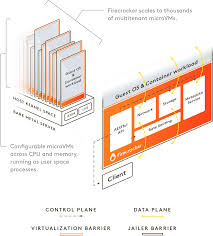
\includegraphics[width=0.8\textwidth]{firecracker.jpeg}
    \end{center}
  \end{columns}
\end{frame}

% Architecture
\section{Architecture}

\begin{frame}{Microservices Architecture}
  \begin{itemize}
    \item Distributed architecture based on independent microservices
    \item Communication via REST APIs And RabbitMQ(AMQP)
    \item Core services:
      \begin{itemize}
        \item \textbf{Python-based services:}
          \begin{itemize}
            \item \textbf{service-cluster}: Host cluster management
            \item \textbf{service-vm-host}: Virtual machine management on hosts
            \item \textbf{service-system-image}: System image management
            \item \textbf{service-vm-offer}: Virtual machine offer management
          \end{itemize}
        \item \textbf{Java-based services:}
          \begin{itemize}
            \item \textbf{service-config}: Configuration management
            \item \textbf{service-proxy}: API gateway and routing
            \item \textbf{service-register}: Service discovery and registration
            \item \textbf{service-user}: User management and authentication
            \item \textbf{service-notification}: Notification system
          \end{itemize}
      \end{itemize}
    \item Automatic service registration via Eureka
  \end{itemize}
\end{frame}

\begin{frame}{Architecture Diagram}
  \begin{center}
    % Placeholder for an architecture diagram
    \includegraphics[width=0.8\textwidth]{Architechture micro-servcice firecracker.drawio.png}
    \caption{IAASFIRECRACKER Microservices Architecture}
  \end{center}
\end{frame}

% Technologies
\section{Technologies Used}

\begin{frame}{Technology Stack}
  \begin{columns}
    \column{0.5\textwidth}
    \textbf{Backend:}
    \begin{itemize}
      \item Python: FastAPI / Flask
      \item Java: Spring Boot / Spring Cloud
      \item SQLAlchemy ORM
      \item MySQL
      \item Firecracker VMM
      \item Eureka (Service Discovery)
    \end{itemize}
    
    \column{0.5\textwidth}
    \textbf{Frontend \& DevOps:}
    \begin{itemize}
      \item Next.js for frontend
      \item Docker / Containerization
      \item API Gateway
      \item Monitoring and Logging
      \item CI/CD Pipeline
    \end{itemize}
  \end{columns}
\end{frame}

% Microservices
\section{Microservices}

\subsection{Python-based Services}

\begin{frame}{service-cluster (Python)}
  \begin{itemize}
    \item Management of physical host clusters
    \item Tracking available resources (CPU, RAM, storage)
    \item Resource allocation for virtual machines
    \item REST API for cluster administration
    \item Interface with service-vm-host
  \end{itemize}
\end{frame}

\begin{frame}{service-vm-host (Python)}
  \begin{itemize}
    \item Virtual machine lifecycle management
    \item Interface with Firecracker VMM
    \item Creation, starting, stopping, and deletion of VMs
    \item VM performance monitoring
    \item Automatic registration with service-cluster
  \end{itemize}
\end{frame}

\begin{frame}{service-system-image (Python)}
  \begin{itemize}
    \item System image management for VMs
    \item Image storage and cataloging
    \item Image versioning
    \item API for image upload and download
    \item Integration with service-vm-host for provisioning
  \end{itemize}
\end{frame}

\begin{frame}{service-vm-offer (Python)}
  \begin{itemize}
    \item Virtual machine offer management
    \item Predefined configuration definitions (CPU, RAM, storage)
    \item Resource pricing
    \item API for browsing and selecting offers
    \item Integration with billing service
  \end{itemize}
\end{frame}

\subsection{Java-based Services}

\begin{frame}{service-config (Java)}
  \begin{itemize}
    \item Centralized configuration management
    \item Environment-specific configuration profiles
    \item Dynamic configuration updates
    \item Configuration versioning and history
    \item Built with Spring Cloud Config
  \end{itemize}
\end{frame}

\begin{frame}{service-proxy (Java)}
  \begin{itemize}
    \item API Gateway implementation
    \item Request routing to appropriate microservices
    \item Load balancing
    \item Request filtering and transformation
    \item Authentication and authorization middleware
    \item Built with Spring Cloud Gateway
  \end{itemize}
\end{frame}

\begin{frame}{service-register (Java)}
  \begin{itemize}
    \item Service discovery and registration
    \item Health checking for registered services
    \item Service metadata management
    \item Load balancing support
    \item Implemented using Netflix Eureka
  \end{itemize}
\end{frame}

\begin{frame}{service-user (Java)}
  \begin{itemize}
    \item User account management
    \item Authentication and authorization
    \item User profile management
    \item Role-based access control
    \item Integration with external identity providers
    \item JWT token generation and validation
  \end{itemize}
\end{frame}

\begin{frame}{service-notification (Java)}
  \begin{itemize}
    \item Event-based notification system
    \item Multiple delivery channels (email, SMS, in-app)
    \item Notification templates
    \item Delivery status tracking
    \item User notification preferences
    \item Integration with messaging queues
  \end{itemize}
\end{frame}

% Features
\section{Features}

\begin{frame}{Main Features}
  \begin{itemize}
    \item On-demand virtual machine creation and management
    \item Selection from predefined system images
    \item Choice of hardware configurations (offers)
    \item Real-time performance monitoring
    \item Usage-based billing
    \item Complete REST API for integration
    \item Swagger documentation for all APIs
    \item Modern Next.js frontend for user interaction
    \item Multi-user support with role-based access control
    \item Event-driven notification system
  \end{itemize}
\end{frame}

% Demonstration
\section{Demonstration}

\begin{frame}{Demonstration}
  \begin{center}
    \huge{System Demonstration}
    
    \vspace{1cm}
    
    \large{Creating and Deploying a Virtual Machine}
  \end{center}
\end{frame}

% Challenges
\section{Challenges Faced}

\begin{frame}{Technical Challenges}
  \begin{itemize}
    \item \textbf{Firecracker Integration:} Configuring and integrating Firecracker with our microservices architecture required significant research and experimentation
    \item \textbf{Network Configuration:} Implementing proper networking between virtual machines and host systems presented complex routing challenges
    \item \textbf{Resource Management:} Developing efficient algorithms for resource allocation across multiple hosts
    \item \textbf{Performance Optimization:} Ensuring near-native performance while maintaining isolation guarantees
    \item \textbf{API Design:} Creating consistent and intuitive APIs across multiple services developed in different programming languages
  \end{itemize}
\end{frame}

\begin{frame}{Development Challenges}
  \begin{itemize}
    \item \textbf{Microservices Coordination:} Managing dependencies and communication between multiple independent services
    \item \textbf{Polyglot Development:} Coordinating development across Python and Java services with different frameworks
    \item \textbf{Testing Complexity:} Creating effective test environments for virtualization technology
    \item \textbf{Documentation:} Maintaining comprehensive documentation across all services
    \item \textbf{Learning Curve:} Team members needed to quickly learn Firecracker technology and microservices best practices
  \end{itemize}
\end{frame}

\begin{frame}{Solutions and Lessons Learned}
  \begin{itemize}
    \item \textbf{Containerization:} Using Docker to standardize development environments across services
    \item \textbf{Service Contracts:} Implementing strict API contracts between services early in development
    \item \textbf{Continuous Integration:} Establishing robust CI/CD pipelines for all services
    \item \textbf{Knowledge Sharing:} Regular technical sessions to share expertise across the team
    \item \textbf{Incremental Development:} Building core functionality first, then expanding features
    \item \textbf{Monitoring:} Implementing comprehensive monitoring from the beginning to identify issues early
  \end{itemize}
\end{frame}

% Conclusion
\section{Conclusion}

\begin{frame}{Conclusion}
  \begin{itemize}
    \item IAASFIRECRACKER provides an open-source alternative to AWS EC2
    \item Modern and scalable microservices architecture
    \item Optimal performance thanks to Firecracker
    \item Ease of use through REST APIs and Swagger documentation
    \item Polyglot implementation with Python and Java services
    \item Modern frontend with Next.js
    \item Next steps: 
      \begin{itemize}
        \item Integration with storage services
        \item Security enhancements
        \item Advanced monitoring and analytics
        \item Expansion of VM template offerings
      \end{itemize}
  \end{itemize}
\end{frame}

\begin{frame}{Questions?}
  \begin{center}
    \huge{Thank you for your attention!}
    
    \vspace{1cm}
    
    \large{Questions?}
  \end{center}
\end{frame}

\end{document}
